Let the graph $U(n)$ denote the Coxeter system generated by $S$, of rank $n$, with minimal relations, i.e.~each distinct pair of generators generates a  $D_\infty$ parabolic subgroup.
Let $\pi \colon F_S \to W_{U(n)}$ denote the projection from the free group to this Coxeter group, let $\overline{w}$ be some choice of pre-Coxeter element in  $F_S$, and let $\overline{R}$ denote all conjugations of $S$ in $F_S$.
As expected, denote the reflections in $W_{U(n)}$ by $R$, which is equal to $\pi(\overline{R})$, and denote $\pi(\overline{w})$ by $w$.
It is known by \cite[Corollary 4.6]{bessis_dual_2006} that $\pi$ is bijective from $\minfact_{\overline{R}}(\overline{w})$ to $\minfact_R(w)$.
Thus, instead of studying $\minfact_{\overline{R}}(\overline{w})$ combinatorially, we can study  $\minfact_R(w)$ using the geometry of this Coxeter complex.
In rank 2,  $W_{U(2)}$ is  $D_\infty$, in all higher ranks  $W_{U(n)}$ is of hyperbolic signature and in particular in rank 3 the arrangement is the Farey tessellation.

\begin{figure}[ht]
	\centering
	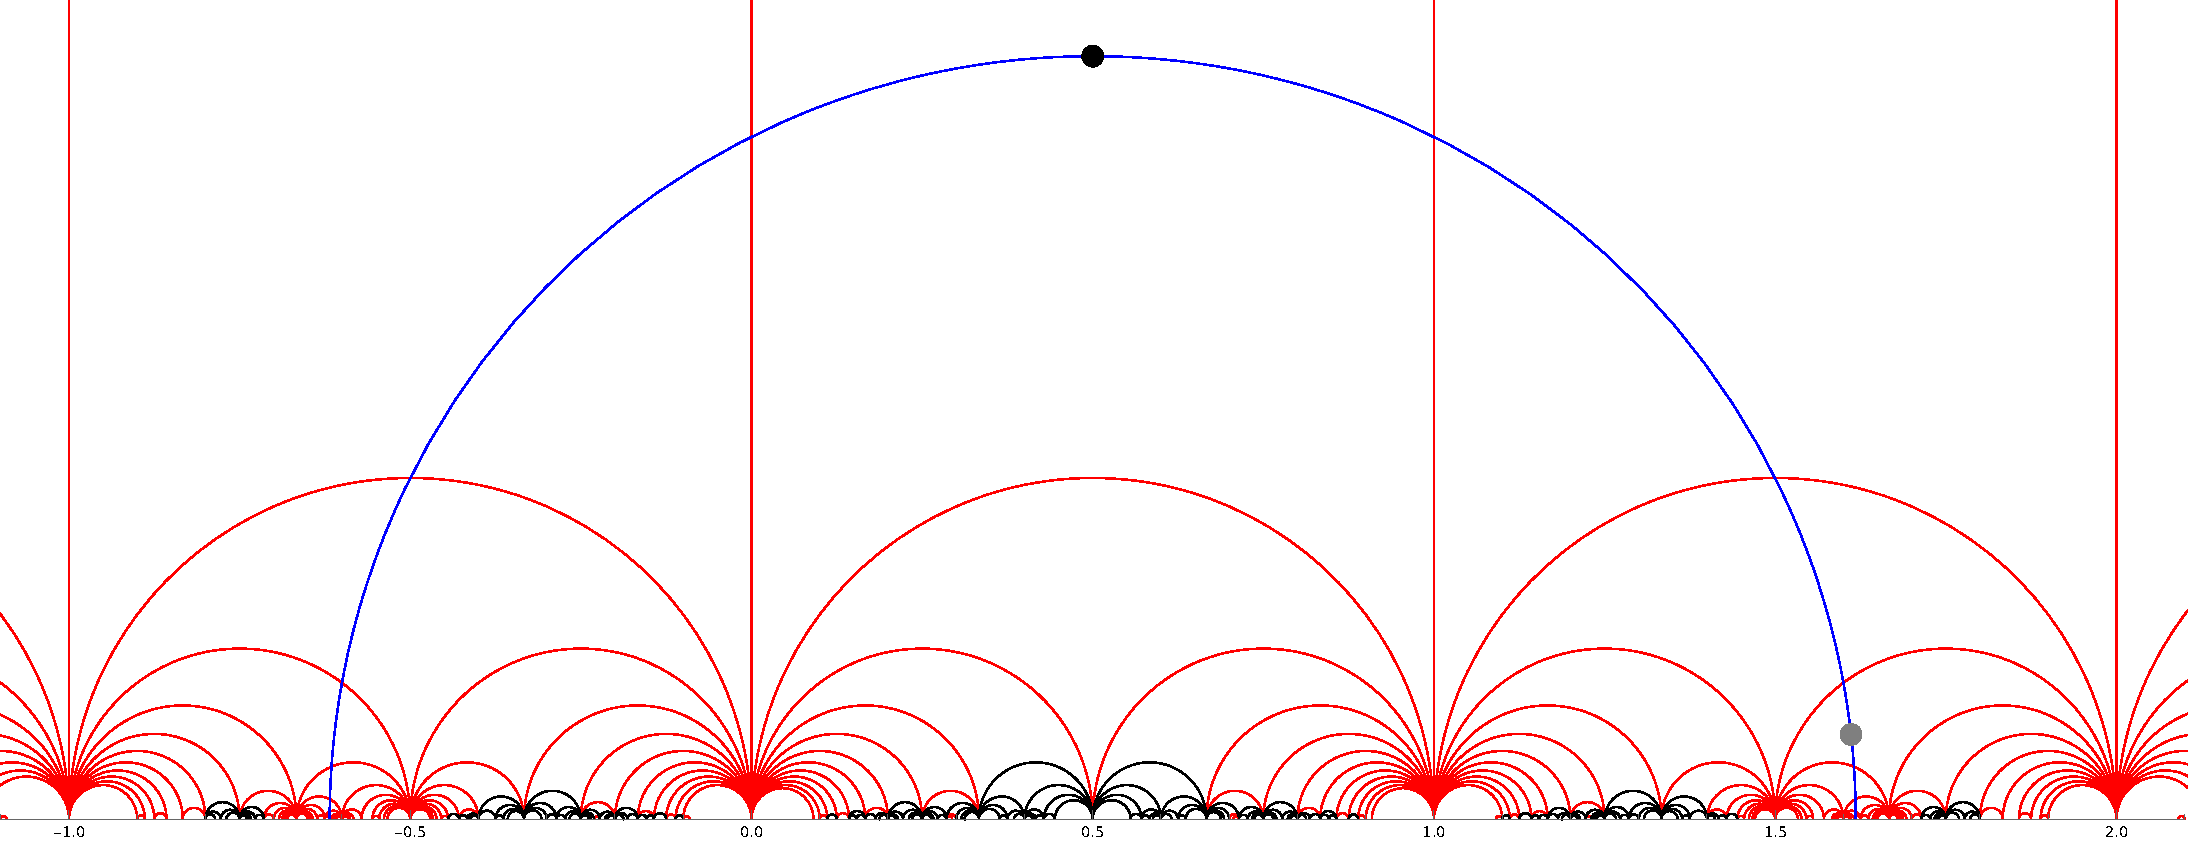
\includegraphics[width=11cm]{infinfinf_QinFareyTesellation.pdf}
	\caption{The Farey tessellation with reflections (geodesics) in $\minfact_R(w)$ highlighted in red.
		This corresponds to the Coxeter element which is reflection in the geodesics connecting $(0,\infty)$,  $(0,1)$ and  $(1,\infty)$ in that order.
		We only looked at factorisations occurring due to the Hurwitz action with words in the braid group of length  $\leq 10$, so we cannot know the accuracy of this picture for sure.
		The Coxeter axis has endpoints at $\frac{1 \pm \sqrt{5}}{2}$ and is shown in blue.
		The Coxeter element moves the black point to the grey point (across 3 cells).}
	\label{fig:Q_in_farey_tesellation}
\end{figure}
\begin{figure}[ht]
	\centering
	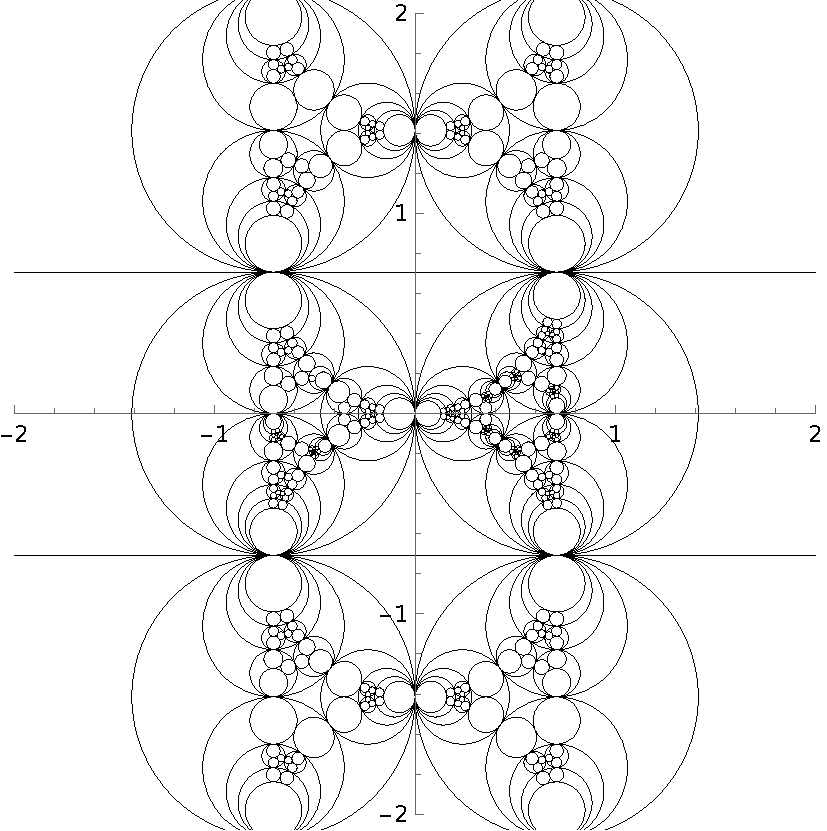
\includegraphics[width=8cm]{3d_farey.pdf}
	\caption{The 3D equivalent of the Farey tessellation corresponds to an arrangement of 4 mutually ideal planes in the disk model of $\Hbb^3$.
		Here we show the intersection of the half-space model of this picture with the boundary plane.
		The picture should be symmetric in reflection in the  $y$-axis and translation in the $y$ direction.
		Anywhere this symmetry is not present is due to rendering limitations.}
	\label{fig:3d_farey_tesellation}
\end{figure}


I have been studying $\minfact_{\overline{R}}(\overline{w})$ in this setting for the last month, and plan to do so for at least another month or so.
A picture of $\minfact_{\overline{R}}(\overline{w})$ in the context of the Farey tessellation is shown in \cref{fig:Q_in_farey_tesellation}, where the Coxeter element $w$ is reflection in the line from  0 to $\infty$, followed by reflection in the line from  $0$ to  $1$, followed by reflection in the line from  $1$ to $\infty$.
In this setting, each reflection is a line connecting two Farey adjacent elements of $\Q \cup \Set{\infty}$, i.e.~a pair in this set.
It is yet unclear whether this geometry can be leveraged in any way to understand this set, but there are clearly some patterns visible in \cref{fig:Q_in_farey_tesellation}.

Ideally, some insight from the rank 3 case could then be applied to the rank 4 case, which is less well understood.
A picture of the rank 4 Coxeter arrangement in the upper half space model (a 3-dimensional equivalent of the Farey tessellation) is shown in \cref{fig:3d_farey_tesellation}.

There are also questions of how the geometry of the Coxeter axis interacts with the Coxeter arrangement in $W_{U(n)}$, and how that translates to other Coxeter systems  $\Gamma$, for which  $W_\Gamma$ is a quotient of  $W_{U(n)}$.
For instance, it seems generally true that a Coxeter element has a cube root, which is a symmetry of the Coxeter arrangement.

After another month of investigating this picture, I plan to move on to a more reading based line of research.
I will study, with the aim of re-writing one of the proofs of, this important paper of Charney and Davis \cite{charney_davis_kpi_1995}.
This should be made more manageable by my previous study of complexes of groups.

After this, I will study in further detail a recent paper of Delucci, Paolini and Salvetti \cite{delucchi_etal_dual_2024}.
This is the most recent example where the dual Artin group was leveraged to answer significant Artin group problems, namely the $K(\pi,1)$ conjecture for $\Gamma$ of rank 3 with hyperbolic signature.
In this paper, the authors show that the so-called interval poset, which we called $C_{w,R}$ in \cref{def:dual_artin}, is a lattice.
It would be very interesting if this could be extended to rank 4 Coxeter systems of hyperbolic signature.
